To round up the section on the \acrlong{pca}, we will look at its applications and these of the \acrlong{svd}.
This way we will get a feeling of possible use-cases and additionally highlight some of their pitfalls.

We will first look at commercial applications that we know to relate to the practicability of \gls{pca}.
Following this, we will see how it can help us to visualise high dimensional data structures.
Then we will look at its applications in the field of computer vision.
Therefore, we will first look at how to compress data sets in a visual example and then visualise how \gls{pca} is used in human face recognition.

Finally, we will raise the awareness of potential pitfalls in \gls{pca} by walking through common mistakes that can be made.


\subsection{PageRank Algorithm}
One famous application of \acrlong{pca} \cite{deisenroth2020mathematics} is the PageRank algorithm proposed by \mycite{page1999pagerank}.
This publication led to the beginning of the Google search engine which demonstrates its efficacy and success.

The primary motivation to build a new search engine arose as the authors saw the lack of success in human maintained lists which failed to keep up with the demands from the rise of the world wide web.
Other attempts such as automated search engines that rely on keywords generally returned unsatisfactory matches.
To make matters worse, both attempts were easy to manipulate by advertisers.
\bigskip


The algorithm, already back in the 1990's, had to deal with hundreds of millions of entries in its data set \cite{brin1998anatomy}.
Simultaneously, it had to answer tens of millions of queries a day.
To achieve such feature, \citeauthor{page1999pagerank} calculate the PageRank using a simple iterative algorithm which corresponds to the principal eigenvectors of the normalised link matrix.
The feasibility of these computations was stated to be possible on medium sized workstations \cite{page1999pagerank}.

To maintain the accurate results, the paper emphasises the importance of crawling and indexing the data as a crucial application of the search engine.
To maintain numerical stability in the search results, the crawled data requires to be precisely parsed across the myriad of HTML structures.

\clearpage

\subsection{Visualisation}
\begin{itemize}
  \item ovarian cancer dataset
  \item about 200 patients
  \item 4000 features
  \item all the same unit
  \item ideal for the problem
  \item 3 dimensions preserve 90\% of the information
  \item Grouping is now visible in a 3D plot
\end{itemize}

\clearpage

\subsection{Compression}
Now we will examine what different compression levels might look like.
For this, we will use a sample image to demonstrate its effects.

\begin{figure}[ht]
    \centering
    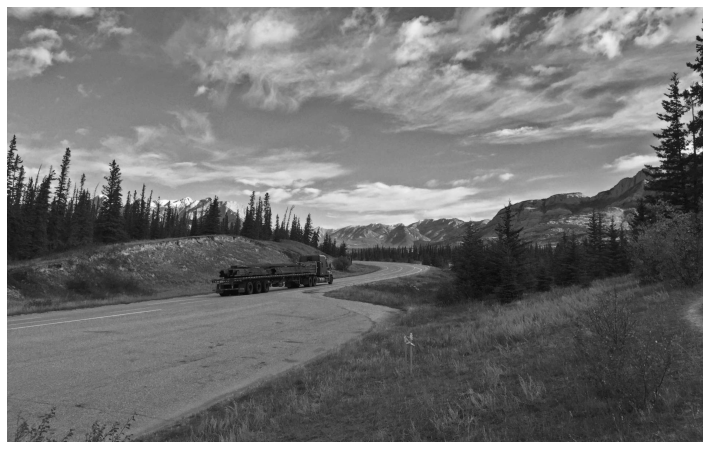
\includegraphics[width=0.725\linewidth]{external_content/media/compression_example/uncompressed.png}
    \captionsetup{justification=centering}
    \caption{Uncompressed image}
    \label{fig:uncompressed}
\end{figure}
\vspace{-2mm}

To begin with, let us consider the uncompressed image in figure \ref{fig:uncompressed} which we will base the compression on.
This image is then translated into an $n \times m$ matrix and decomposed using the \gls{svd}.

After computing the \gls{svd}, we will examine the output when considering various $r$ \acrlongpl{pc} in figure \ref{fig:compressionComparison}.
A compression down to the first 10 \glspl{pc} in figure \ref{fig:compressionNX} shows a considerable decrease in quality.
For this representation we require about 0.8\% of the original data storage.
\medskip

Next up we have chosen the first 50 \glspl{pc} in figure \ref{fig:compressionNL}.
The thumbnail already looks recognisable, meanwhile zooming in does show significant qualitative downturns.
This compression requires 4\% of the original data size.

Finally, when looking at $r=120$, or 10\% of the original data size, we can still observe some noise in the picture but retain the full level of detail.


% \item Talk about grouping similar areas
% \item Compression example
% \item logplot which shows how much variance is preserved

\begin{figure}[h]
  \centering
  \begin{subfigure}{0.32\textwidth}
      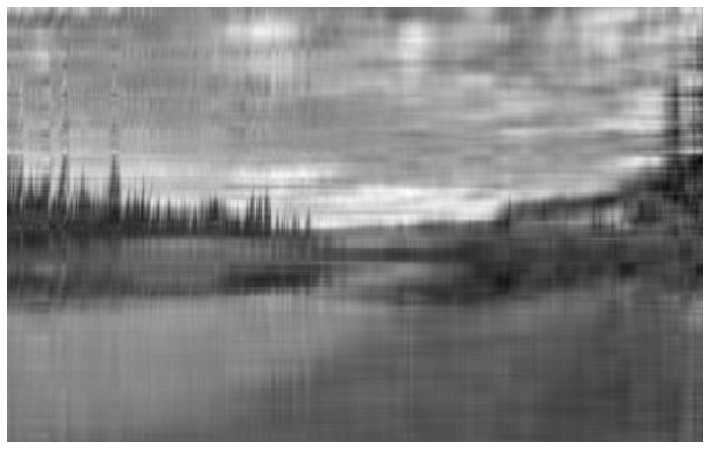
\includegraphics[width=\textwidth]{external_content/media/compression_example/n=10.png}
      \caption{$r$ = 10}
      \label{fig:compressionNX}
  \end{subfigure}
  \hfill
  \begin{subfigure}{0.32\textwidth}
      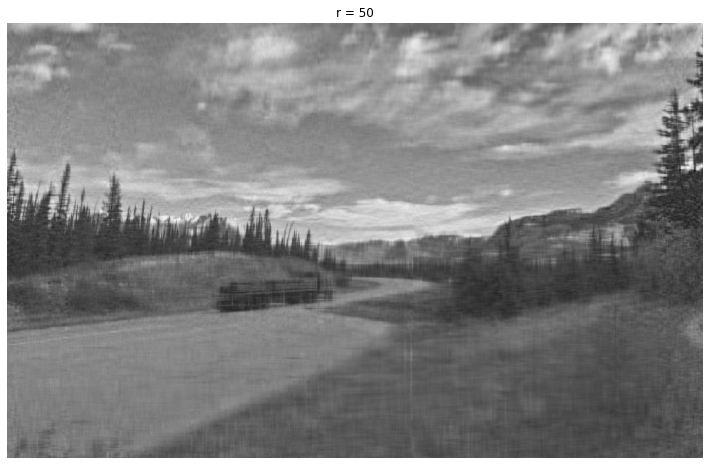
\includegraphics[width=\textwidth]{external_content/media/compression_example/n=50.png}
      \caption{$r$ = 50}
      \label{fig:compressionNL}
  \end{subfigure}
  \hfill
  \begin{subfigure}{0.32\textwidth}
      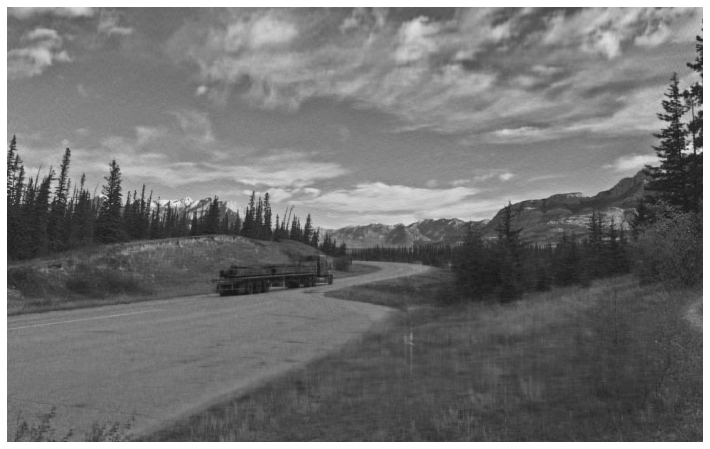
\includegraphics[width=\textwidth]{external_content/media/compression_example/n=120.png}
      \caption{$r$ = 120}
      \label{fig:compressionNC}
  \end{subfigure}
  \caption{Comparison of different compression levels}
  \label{fig:compressionComparison}
\end{figure}

\clearpage

\subsection{Eigenfaces} \label{sec:eigenfaces}
\begin{center}
    \begin{figure}[h]
      \centering
      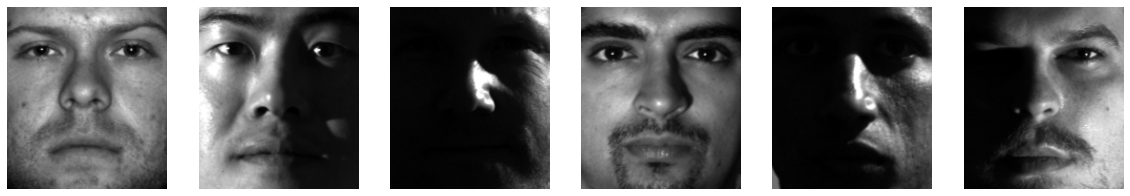
\includegraphics[width=0.86\linewidth]{external_content/media/eigenfaces.png}
      \captionsetup{justification=centering}
      \caption{Samples from the Eigenfaces data set \cite{georghiades2001few}}
      \label{fig:eigenfaces}
    \end{figure}
\end{center}
\vspace{-8mm}


\begin{minipage}[h][120mm][t]{0.35\linewidth}
    \begin{center}
        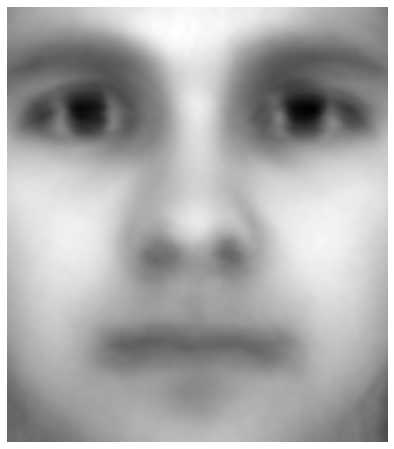
\includegraphics[width=0.81\linewidth]{external_content/media/eigenfaces/average_face.png}
        \captionsetup{justification=centering,type=htypei}
        \captionof{figure}{Average face}
        \label{fig:eigenfaceAVG}
    \end{center}
    \begin{center}
        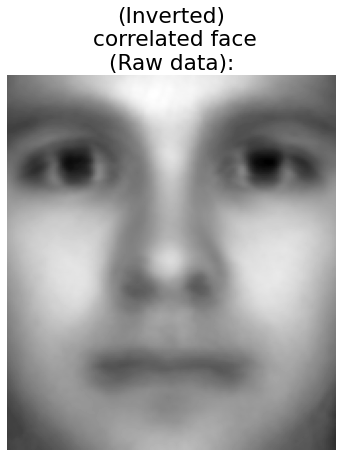
\includegraphics[width=0.81\linewidth]{external_content/media/eigenfaces/correlated_face-uncentered.png}
        \captionsetup{justification=centering,type=htypei}
        \captionof{figure}{Correlated face\\on uncentered data}
        \label{fig:eigenfaceCORRuncentered}
    \end{center}
    \begin{center}
        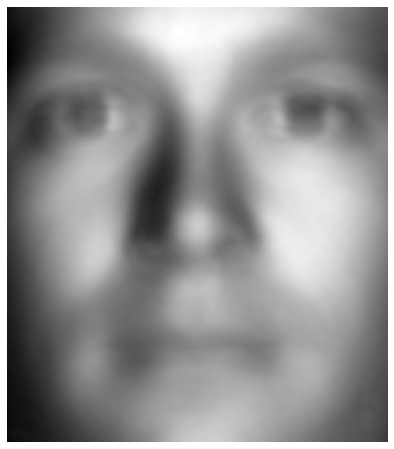
\includegraphics[width=0.81\linewidth]{external_content/media/eigenfaces/correlated_face-centered.png}
        \captionsetup{justification=centering,type=htypei}
        \captionof{figure}{Correlated face\\on centred data}
        \label{fig:eigenfaceCORR}
    \end{center}
\end{minipage}\hfill%
\begin{minipage}[h][120mm][t]{0.55\linewidth}

    % reset indentation
    \setlength{\parindent}{2em}

    \bigskip

    \noindent
    For this demonstration, we will introduce the Yale Face Database.
    The data set as presented contains 2282 faces from 36 people under different lighting conditions.
    A few samples are depicted in figure \ref{fig:eigenfaces}.
    This data set will be the basis for the examples in the upcoming sections.

    \bigskip

    In figure \ref{fig:eigenfaceAVG} we see what the average of all faces looks like.
    We can observe blurriness in the transitions in selected areas where differences in facial traits are most distinctive such as the contours of the face or the edge of the nose.

    \medskip

    Meanwhile, the next image results from computing the correlation matrix on uncentered data.
    Figure \ref{fig:eigenfaceCORRuncentered} looks nearly identical to the average face in figure \ref{fig:eigenfaceAVG}.
    The key difference is that the transitions areas appear darker instead of blurred.

    \medskip

    On the other hand, the correlated face on the centred data in figure \ref{fig:eigenfaceCORR} illustrates the data from a new perspective.
    We can observe that centring the data has given new opportunities, whether these are for better or for worse remains to be determined according to the circumstances of a given problem.

    % \item Difference centered and non-centered data
    % \item average face

\end{minipage}%

\clearpage

\subsection{Pitfalls}
\subsubsection{Misaligned Data}


\begin{wrapfigure}[14]{r}{0.5\textwidth}
    \centering
    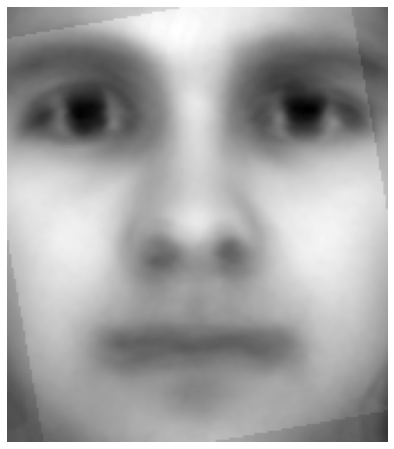
\includegraphics[width=0.9\linewidth]{external_content/media/rotation/average_face-rotation.png}
    \captionsetup{justification=centering}
    \caption{Misaligned eigenface}
    \label{fig:misalignedEigenface}
\end{wrapfigure}

One major problem with \gls{pca} originating from the \gls{svd}, is that the units of the data on all axes as well as its alignment significantly impacts the resulting decomposition \cite{brunton2019data}.
The demonstration of the eigenfaces solely showcased solid results because the faces have been meticulously centred and cropped manually prior to the evaluation.
The impact can be observed in the adjoining figure \ref{fig:misalignedEigenface}.

To demonstrate this issue, 190 of the 2282 faces have been rotated by 10\textdegree\ prior to the \gls{svd}.
This shows that a mere 8\% of corrupted data is enough to obfuscate the analysis.


% \cite{brunton2019data} (section 1.7)

% \item Showcase Eigenfaces with rotation
% \item only few images ruin the batch
% \item the data set was meticulously centered and optimized by hand for a proof of concept


\subsubsection{Different units}

\begin{figure}[h]
    \centering
    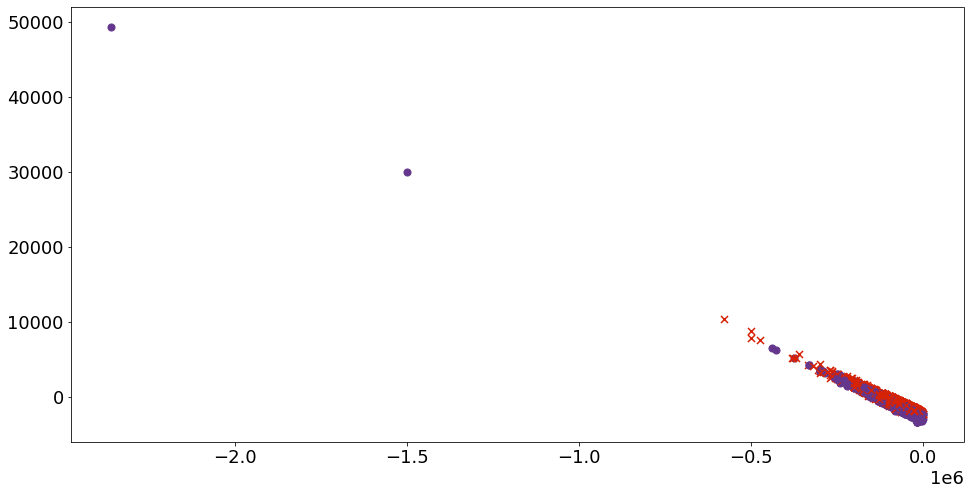
\includegraphics[width=0.8\linewidth]{external_content/media/wrong_units/graph.png}
    \captionsetup{justification=centering}
    \caption{Unit mismatch}
    \label{fig:unitMismatch}
\end{figure}

\noindent
Now we want to showcase what happens when \gls{pca} is applied on a data set with unrelated units.
This examination is based on a \href{https://www.kaggle.com/nehalbirla/vehicle-dataset-from-cardekho?select=Car+details+v3.csv}{vehicle data set} with which we tried to identify patterns in terms of final selling price.
As we can see in figure \ref{fig:unitMismatch}, the graph hardly expresses any useful information.


% Different units WITHIN THE MATRIX... \cite{Jolliffe2002book} (Section 2.3 page 22)

% \item relevant for ALL the values
% \item bigger numbers become dominant no matter what
% \item example car data set. I thought I was being smart... NOPE





\clearpage




\subsubsection{Too broad singular values}

For our last examination we will showcase the effects an adequate choice of \acrlong{pc} has on the resulting evaluation.
We are now considering the Yale Face Database again and comparing two exemplary \glspl{pc} of two people.

\begin{center}
    \begin{figure}[h]
      \centering
      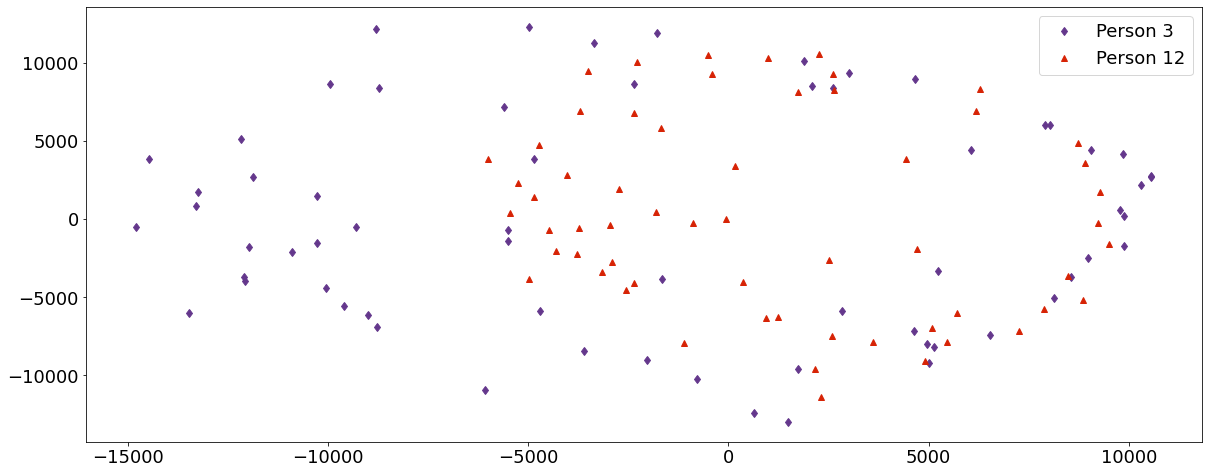
\includegraphics[width=0.9\linewidth]{external_content/media/choice_of_pc/p3_12-pc1_2-centered.png}
      \captionsetup{justification=centering}
      \caption{First two principal components for person 3 and 12}
      \label{fig:pcIandII}
    \end{figure}
\end{center}

\vspace{-8mm}
For the first evaluation in figure \ref{fig:pcIandII}, we are considering the two major \glspl{pc} when naively picking the highest singular values.
Each point represents one image from the respective person.
As we can observe, the assertions made from the graph are negligible.
This is due to the \glspl{pc} primarily picking up the biggest similarities in the pictures such as the lighting conditions.

But this does not have to be the end, upon further inspection by trial and error, we can identify \gls{pc} 5 and 6.
Said \gls{pc} propose a split of the graph seen in figure \ref{fig:pcVandVI}.
The values are now heterogenous and we can make certain observations and draw conclusions based on their location within the clusters.

\begin{center}
    \begin{figure}[h]
      \centering
      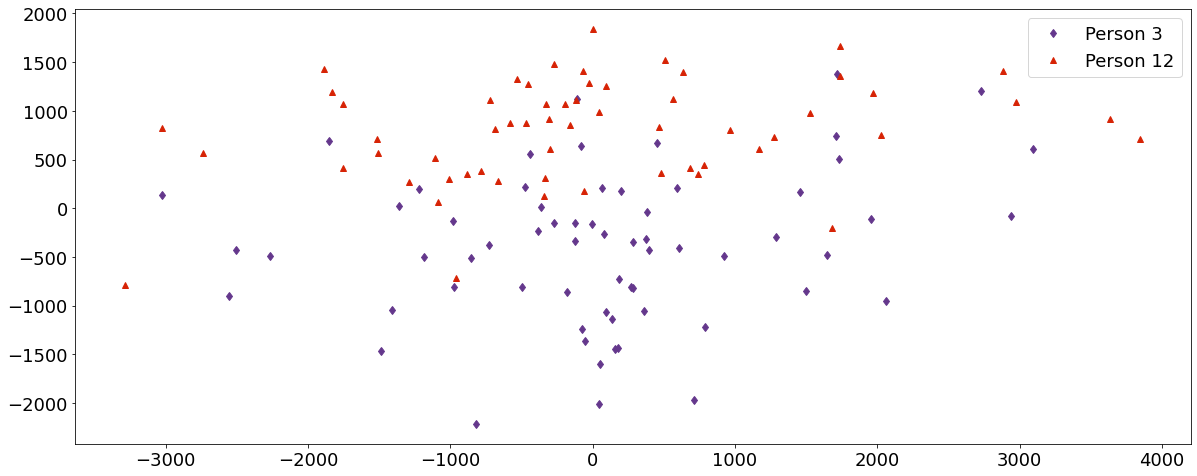
\includegraphics[width=0.9\linewidth]{external_content/media/choice_of_pc/p3_12-pc5_6-centered.png}
      \captionsetup{justification=centering}
      \caption{\gls{pc} 5 and 6 for person 3 and 12}
      \label{fig:pcVandVI}
    \end{figure}
\end{center}

% First principal components might be too general and not \cite{brunton2019data} (section 1.6 - last figure)

% \item Showcase Eigenfaces distribution of the images
% \item 5 and 6 work great
% \item others ruin all the information
% \item all the vertices are one picture of a person
% \item taken with various facial expressions and very different lighting settings

\clearpage

\clearpage
